\chapter{\protect Results and Discussions}

According to Grundy et al. (2016), CH$_4$ from Pluto may accumulate by cold-trapping, onto surface of Charon. The amount of CH$_4$ varies throughout the surface of Charon because it depends on duration of temperature below 25 K. The duration depends on diurnal motion and thermal inertia of Charon. With a tilted axis of 112 degrees to the ecliptic, higher concentration of CH$_4$ will accumulate at the pole (see chapter 1 for details). Therefore, we investigate different concentrations of CH$_4$+NH$_3$ ice mixtures and answer several questions: Will different concentration of CH$_4$ mix with high concentration of ammonia observed on crater position and throughout the surface of Charon (Grundy et al. 2016) have structure difference in accumulation of tholin? Are there variations of photo-products when concentration of CH$_4$ differ during warm-up? Since both EUV and VUV irradiation irradiates onto Charon, are there any differences when we change the photon source from VUV to EUV to irradiate the ice mixtures?\\

The main source to irradiate the dark side of Charon is Lyα reflected by interplanetary medium (Grundy 2016). Other sources such as the energetic ions in solar wind, consists of mainly H$^+$, He$^+$, He$^{++}$ and O$^{2+}$ etc are originated from solar corona or IPM. These ions would also reflect solar irradiation to the dark side of Charon. Among these irradiations, we picked He II irradiation because He II is 3 – 20 times more intense then He I during a solar flare. As it varies, it is difficult to estimate the dose onto Charon. Besides, electronic flux is also present in solar wind but it is one order of magnitude lower than proton flux. The flux for energetic electrons observed at the 1 A. U. position is available (http://www.swpc.noaa.gov/products/goes-electron-flux). Although electron flux is much less important than Lyα, and their flux varies, we also compare the electron irradiation experiment done by Kim and Kaiser (2011) on CH$_4$+NH$_3$ ice mixtures in this chapter. \\

When Charon is shine by direct sun light, the surface temperature increases and deliver the heat to the poles by conduction. From the model of Grundy et al. (2016), the surface temperature of the pole area would increase to 60 K that the heating rate depends on the thermal conductivity of Charon. To demonstrate the heating process, we warmup our ice mixture with a heating rate 1 K/min and monitor the ice by both QMS and scanning IR spectra with 5 K intervals. We will look into whether there are new species formed during warmup and monitor the gas phase desorption.\\

Finally, in this chapter, after we focus on the concentration effect of CH$_4$ on photo-products, photon energy effects, species detected during warmup phases, we present the residues accumulated by irradiating CH$_4$+NH$_3$ ice mixtures with different ratios. Since both tholin formed on Titan and Charon has similar colour, we also compare the IR spectra of MDHL, NSRRC with different configurations with the residues on Titan with experiments done by Imanaka et al.\\
\section{The infra-red spectrums and peaks identification}
Before and after deposition, we scanned an IR spectrum and plotted the absorbance of the ice mixtures. Figure \ref{fig:widerange} is a plot of the absorbance of the CH$_4$+NH$_3$ ice mixtures in different ratios of CH$_4$+NH$_3$ ice mixtures, from top to bottom 1:20, 1:10, 1:5 and 3:2. We have labelled the peaks which we used to calculate the column densitiesby dotted lines throughout the graph. Main products we have detected are C$_2$H$_6$, CN$^-$ and C$_3$H$_8$. The peak positions with the references are listed in Table \ref{tab:WavenumberMDHL}.\\

\begin{figure}
\centering
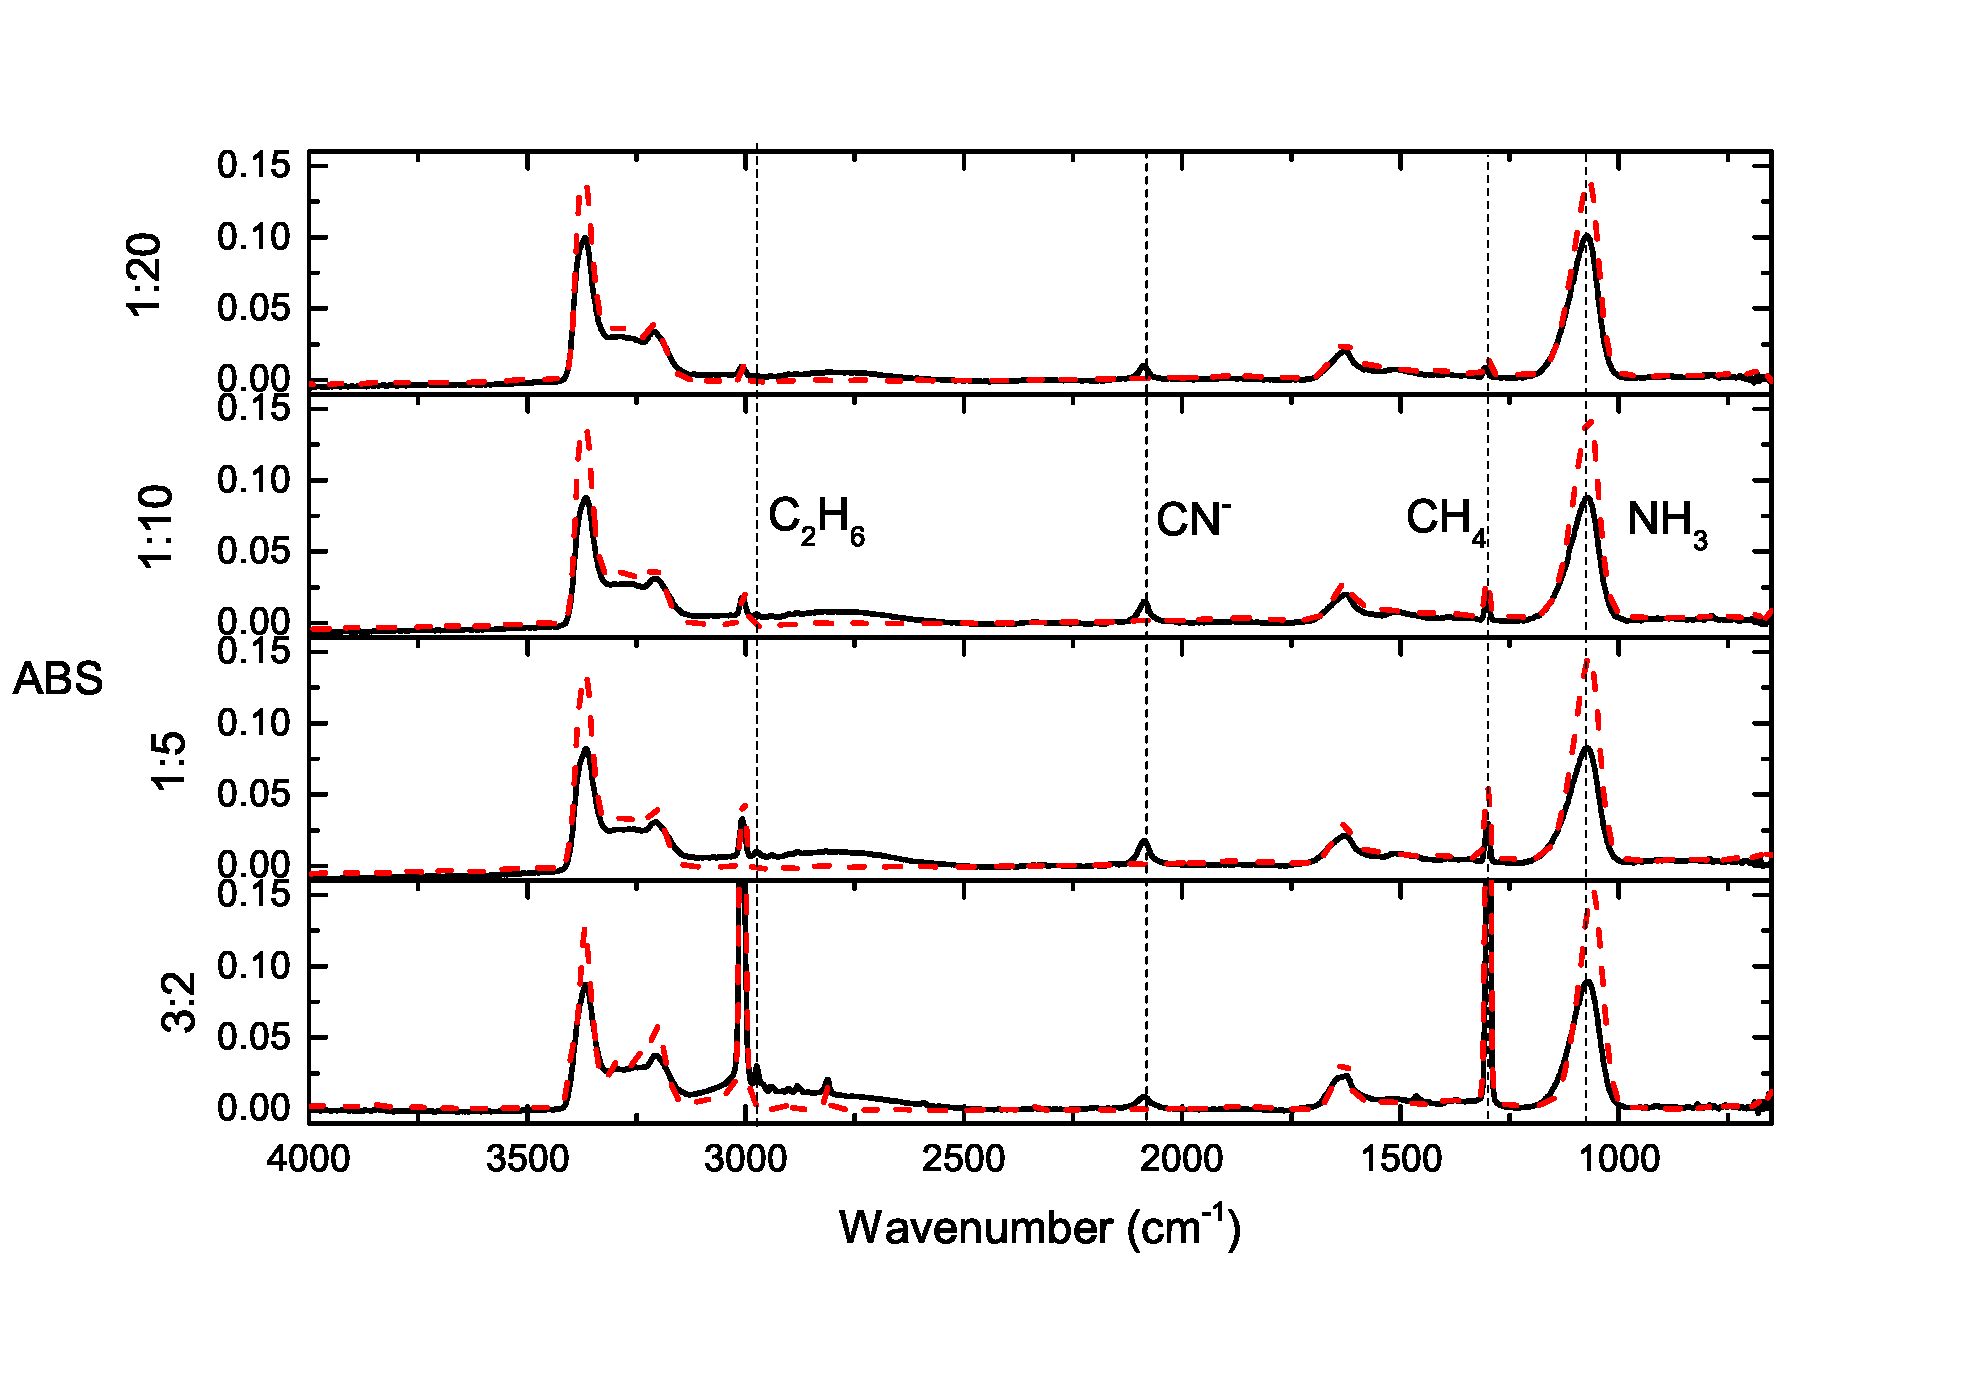
\includegraphics[width=\textwidth]{figures/chapter3/widerange.eps}
\caption{The the infra-red spectrum of CH$_4$ + NH$_3$ ice mixtures before irradiation (dashed) and VUV irradiated ice mixtures provided by MDHL. }
\label{fig:widerange}
\end{figure}

\begin{table}[htbp]
\caption{The peak positions of identified substances after irradiation in different configurations of ice mixtures.}
\label{tab:WavenumberMDHL}
\begin{tabular}{ccccccc}
\hline
\hline
\multicolumn{2}{c}{Literture assignments} & \multicolumn{4}{c}{CH$_4$+NH$_3$ ratio (MDHL)} &  \\
\hline
Wavenumber & Carrier  & 1:5  & 1:10  & 1:20  & 3:2  & Ref. \\
(cm$^{-1}$) &   & (cm$^{-1}$) & (cm$^{-1}$) & (cm$^{-1}$) & (cm$^{-1}$) &\\
\hline
3375 & $\nu_3$ (NH$_3$) & 3366 & 3366 & 3369 & 3367 & 1 \\
3290 & $2\nu_4$ (NH$_3$) & - & - & - & - & 1 \\
3210 & $\nu_1$ (NH$_3$) & 3207 & 3208 & 3210 & 3205 & 1 \\
3011 & $\nu_3$ (CH$_4$) & - & - & - & - & 2 \\
2972 & $\nu_{10}$ (C$_2$H$_6$) & 2975 & - & - & 2975 & 3 \\
2960 & C$_3$H$_8$ & - & - & - & 2960 & 7 \\
2941 & $\nu_8+\nu_11$ (C$_2$H$_6$) & 2940 & - & - & 2940 & 3 \\
2904 & $\nu_1$ (CH$_4$) & 2901 & - & - & 2901 & 5 \\
2879 & $\nu_5$ (C$_2$H$_6$) & 2882 & 2883 & - & 2882 & 3 \\
2814 & $\nu_2+\nu_4$ (CH$_4$) & - & - & - & 2815 & 5 \\
2083 & $\nu$ (CN$^-$) & 2088 & 2087 & 2088 & 2088 & 2 \\
1625 & $\nu_4$ (NH$_3$) & 1625 & 1625 & 1626 & 1631 & 1 \\
1514 & $\delta$ (NH$_2$) & 1509 & 1507 & 1505 & 1511 & 6 \\
1465-1440 & deform CH$_2$ scissor & 1461 & - & - & 1463 & 3,4 \\
1390-1370 & CH$_3$ sym deform & 1394 & 1394 & 1394 & 1372 & 4 \\
1298 & $\nu_4$ (CH$_4$) & 1301 & 1302 & 1305 & 1299 & 2 \\
1075 & $\nu_2$ (NH$_3$) & 1073 & 1072 & 1072 & 1072 & 1 \\
820 & $\nu_12$ (C$_2$H$_6$) & - & - & - & 820 & 3 \\
\hline
\end{tabular}\\
Reference: 1. Bossa et al 2008 2. Moore and Hudson 2003 3. Kim et al. 2010 4. Socrates 2001 5. Bennet and Kaiser 2007 6. Zheng et al. 2008 7. Hudson and Moore 2004
\end{table}


We integrated the area and divided by the absorption strength stated in table 3.2. Although we understand that there is an average error in absorption strengths of no more than 10 \%  when the pure ice is diluted in N$_2$ and H$_2$O (Richey and Gerakines 2012). In our case, absorption strengths changes after CH$_4$ and NH$_3$ are mixed. For example, according to d' Hendecourt and Allamandola (1986), the band of NH$_3$ located at 1070 cm$^{-1}$ would not change much (from $1.1 \times 10^{-17}$ to $1.2 \times 10^{-17}$) when excess water is added to pure NH$_3$ and therefore, we may use the same absorption strength throughout our discussion to give a brief concept on what is the column density of the species and how is the absorption area changes when concentrations of ice mixtures and photon energy are changed. For the case of CN$^-$, we know that CN$^-$ has a bond order =3 by its molecular orbitals which is different from CN stretching (bond order 2.5) which is very sensitive to the matrix environment. As an example, by Borget et al. (2012), the CN stretch in amino acetonitrile change by factor of 2 between the pure molecule itself and in a mixture of amino acetonitrile and H$_2$O (1:3). Here, we adopt the absorption strengths stated in Table \ref{tab:Absorbance} and neglect the error in absorption strengths.\\

\begin{table}[htbp]
\caption{The strength of absorbance adopted in this thesis measured in literatures of pure ice samples}
\label{tab:Absorbance}
\begin{tabular}{cccccc}
\hline
\hline
Wavenumber (cm$^{-1}$) & Assignment  & Vibration & FWHM & A value ($\times 10^{-17}$) & Reference \\
\hline
2976 &  C$_2$H$_6$ & -CH$_3$ & - & 1.05 & 2 \\
2960 & C$_3$H$_8$ & -CH$_2$- & - & 2.58 & 2 \\
2086 & CN$^-$ & CN & - & 1.8 & 3 \\
1297 & CH$_4$ & CH deformation & 8 & 0.61 & 1 \\
1070 & NH$_3$ & "umbrella mode" & 68 & 1.7 & 1 \\
\hline
\end{tabular}
Reference: 1. d'Hendecourt and Allamandola (1986) 2. Moore and Hudson (1998) 3. Noble et al. (2013)
\end{table}

\section{Reaction mechanisms}

\subsection{C$_2$H$_6$}

\begin{figure}
\centering
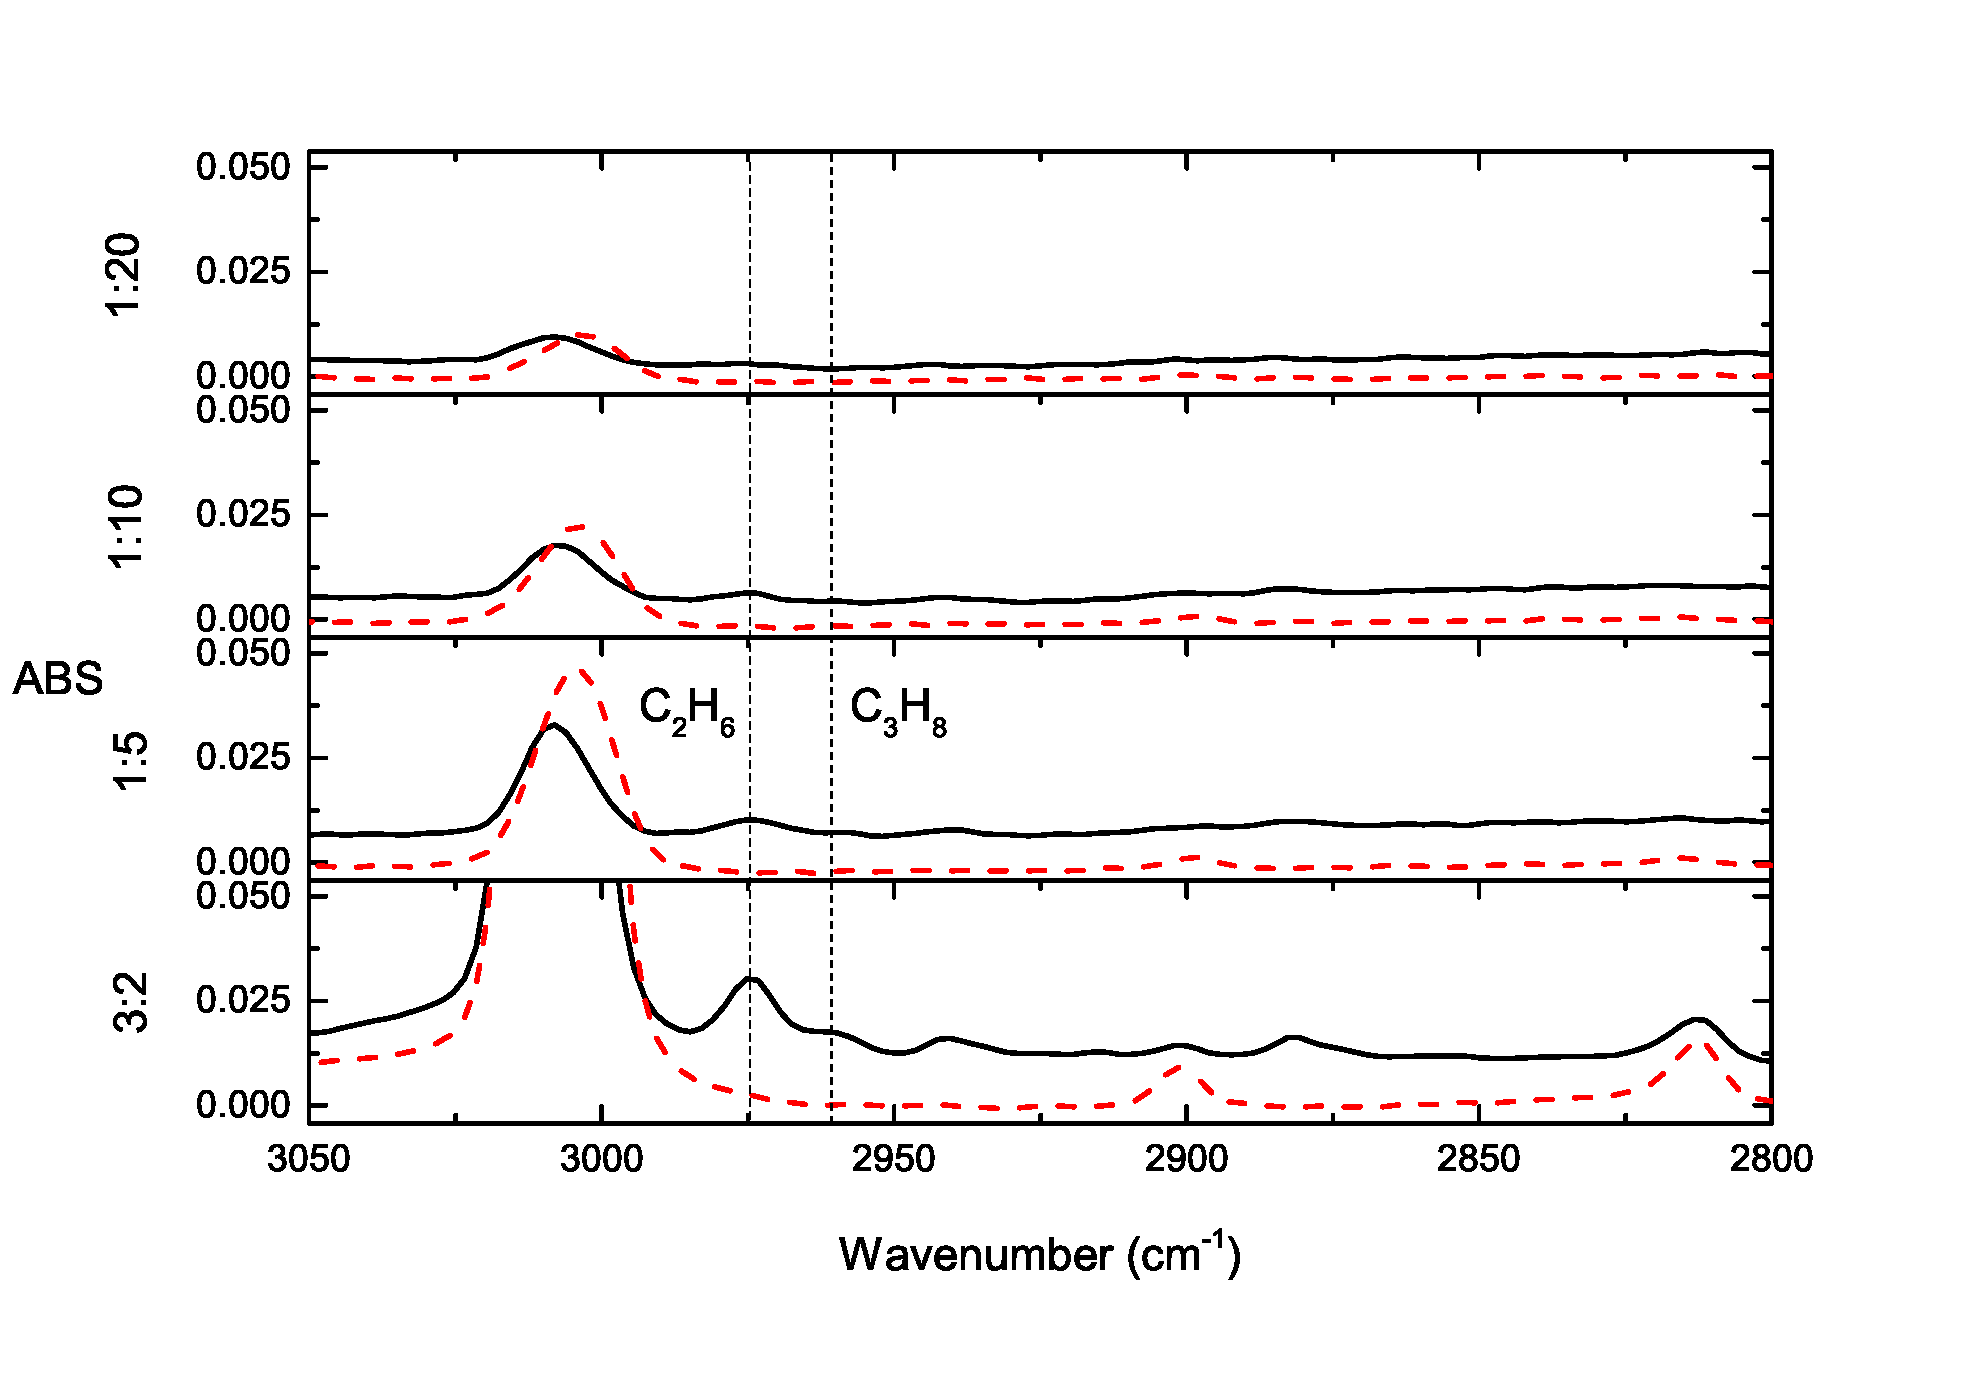
\includegraphics[width=\textwidth]{figures/chapter3/C2H6.eps}
\caption{The the infra-red spectrum of CH$_4$ + NH$_3$ ice mixtures of C$_2$H$_6$ and C$_3$H$_8$ before irradiation (dashed) and VUV irradiated ice mixtures provided by MDHL. }
\label{fig:C2H6}
\end{figure}

The assignment of C$_2$H$_6$ is confirmed by several bands listed in table \ref{tab:WavenumberMDHL}. Figure \ref{fig:C2H6} is a partial of figure \ref{fig:widerange}. The absorption peak located at 2075 cm$^{-1}$ is the strongest vibration of C$_2$H$_6$. The formation mechanism of C$_2$H$_6$ in astrophysical environment is proposed by Bennet et al. (2006), that the main route to form C$_2$H$_6$ is by a combination of 2 CH$_3$ radicals (equation \ref{eq:CH3} and \ref{eq:C2H6}):

\begin{equation}
CH_4 + hv \rightarrow CH_3
\label{eq:CH3}
\end{equation}
\begin{equation}
2 CH_3 \rightarrow C_2H_6
\label{eq:C2H6}
\end{equation}

The energy required to produce 1 CH$_3$ radical from CH4 is 4.42 eV. 2 CH$_3$ radicals recombine to form C$_2$H$_6$ releases 3.74 eV. Therefore, equation \ref{eq:C2H6} is a no-barrier exothermic process. However, C$_2$H$_6$ is not detected in CH$_4$+NH$_3$=1:20 ice mixtures. Figure \ref{fig:lab_C2H6} shows the temporal formation column density of C$_2$H$_6$ in different configurations of irradiated ice mixtures.  As the formation only depends on CH$_4$, we may use first order kinetics equation to fit the column density versus photon dose.
\begin{equation}
[A] = [A]_0(1 - e^{-k_1 t})
\label{eq:1step}
\end{equation}
to fit the formation of C$_2$H$_6$. The fitting results are shown in table \ref{tab:fittingC2H6}.

\begin{figure}
\centering
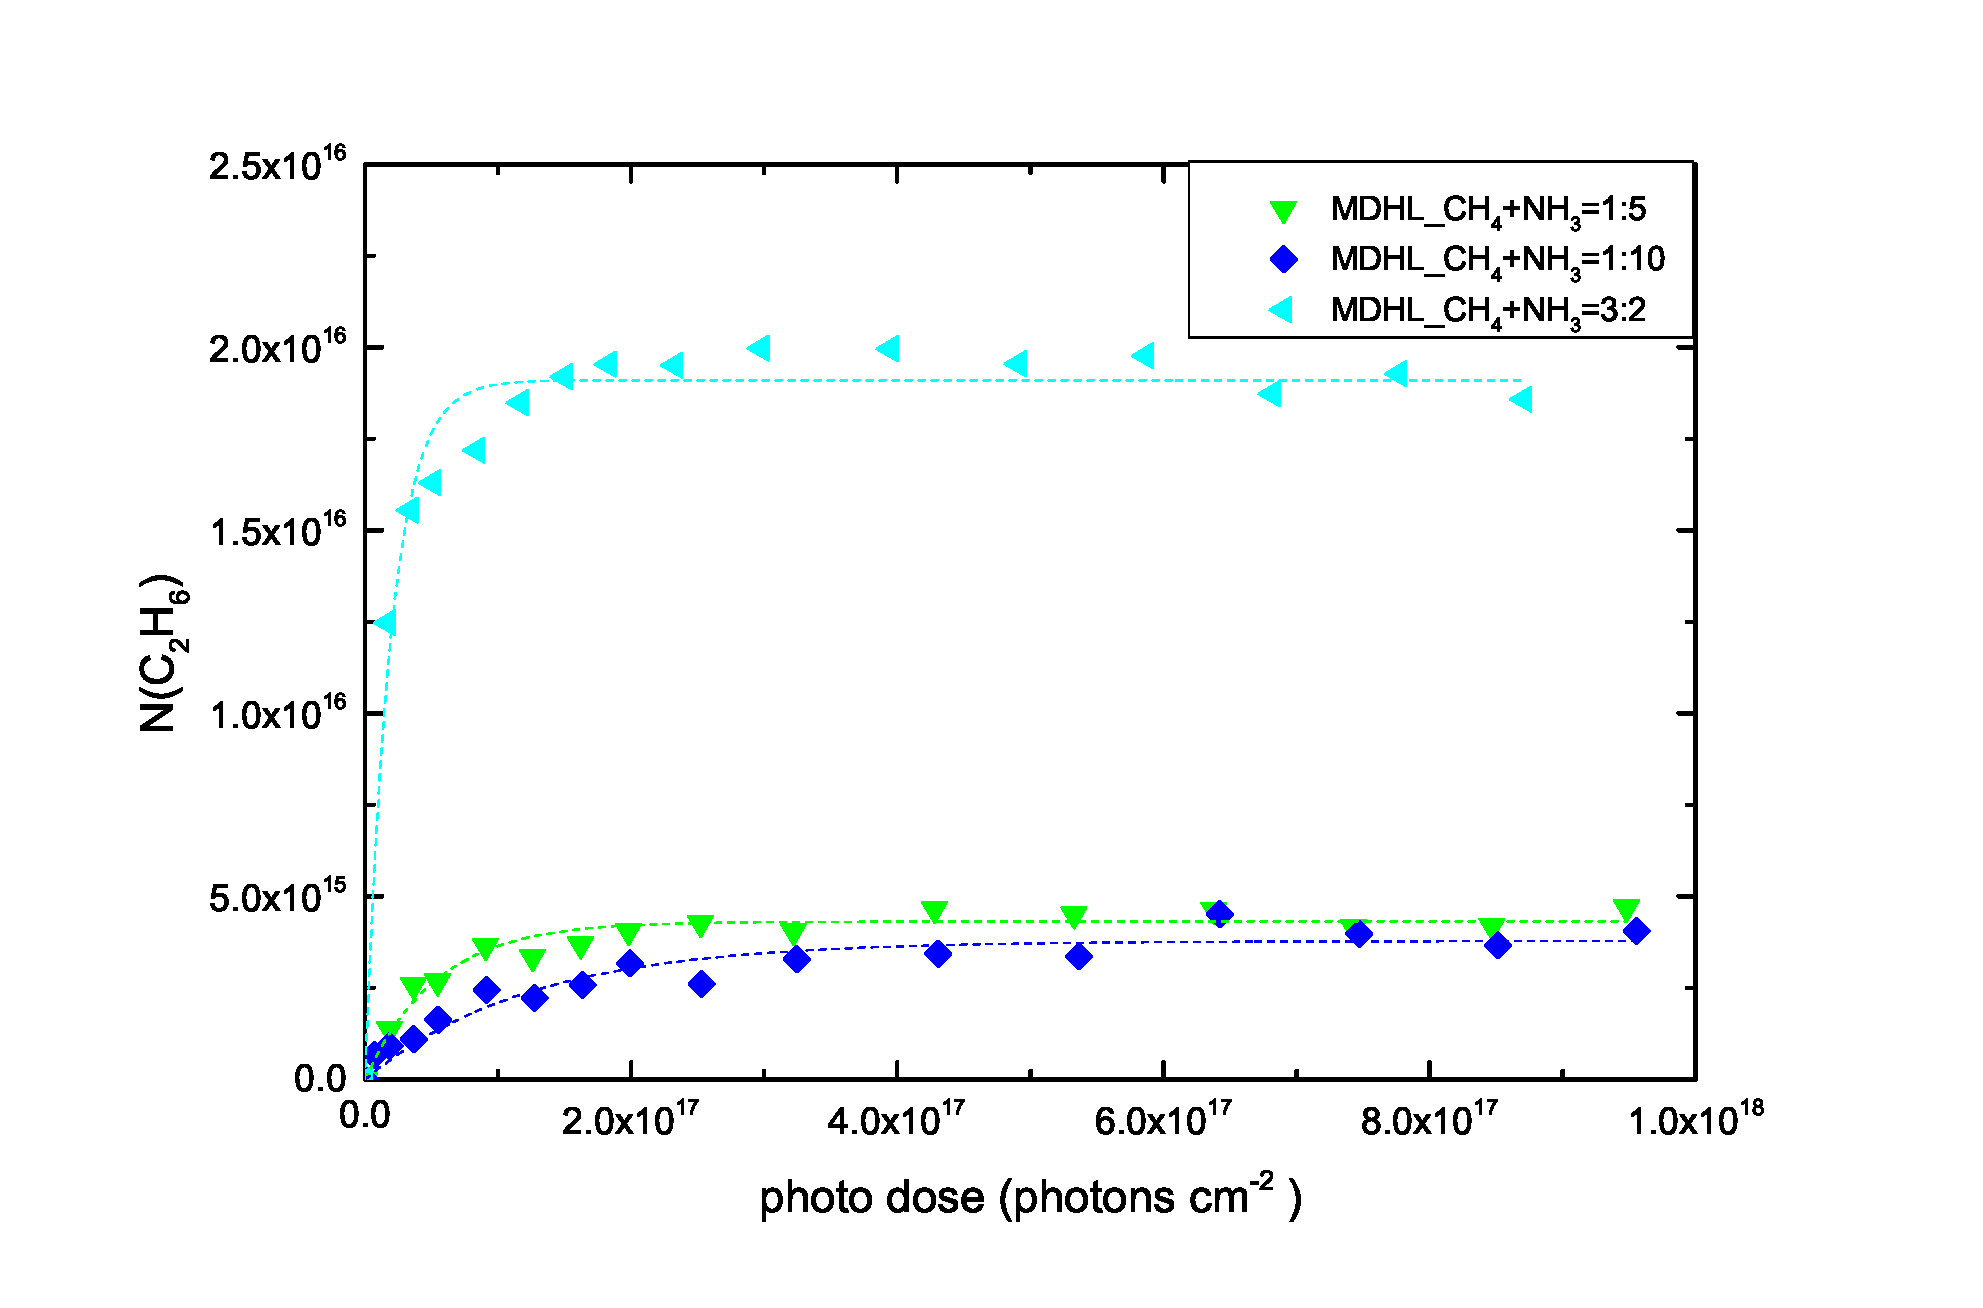
\includegraphics[width=\textwidth]{figures/chapter3/Lab_C2H6.eps}
\caption{The column density of C2H6 during CH4 + NH3 ice mixtures irradiated by MDHL. }
\label{fig:lab_C2H6}
\end{figure}

\begin{table}[htbp]
\caption{The fitting results of C$_2$H$_6$ by [C$_2$H$_6$]=[C$_2$H$_6$]$(1 - e^{-k_1 t})$}
\label{tab:fittingC2H6}
\begin{tabular}{ccc}
\hline
\hline
Ratio of CH$_4$+NH$_3$ & A (x10$^{15}$ molecules cm$^{-2}$) & k (x10$^{-17}$ photon$^{-1}$) \\
\hline
1:10 & 2.90 $\pm$ 1.25 & 0.92 $\pm$ 0.15 \\
1:5 & 4.16 $\pm$ 0.28 & 2.28 $\pm$ 0.28 \\
3:2 & 19.2 $\pm$ 0.15 & 5.28 $\pm$ 0.25 \\
\hline
\end{tabular}
\end{table}

From table \ref{tab:fittingC2H6}, production rate is also proportional to the initial CH$_4$ concentration.


\subsection{C$_3$H$_8$}

The peak positioned at 2960 cm$^{-1}$ belongs to –CH$_2$- so we assigned that as C$_3$H$_8$, as the shortest carbon chain. The signal to noise ratio in CH$_4$+NH$_3$ = 1:10 is poor that we can not quantize the amount of C$_3$H$_8$ (figure \ref{fig:C2H6}).

It is a secondary product formed by a combination of either C$_2$H$_6$ + CH$_2$ (equation \ref{eq:C3H81})or C$_2$H$_4$ + CH$_4$ (equation \ref{eq:C3H82}).
\begin{equation}
C_2H_6 + CH_2 \rightarrow C_3H_8
\label{eq:C3H81}
\end{equation}
\begin{equation}
C_2H_4 + CH_4 \rightarrow C_3H_8
\label{eq:C3H82}
\end{equation}

By modern peak fitting method, we deconvoluted the overlapped C$_2$H$_6$ and C$_3$H$_8$ into two gaussians.

\subsection{CN$^-$}

\begin{figure}
\centering
\includegraphics[width=\textwidth]{figures/chapter3/CN.eps}
\caption{The the infra-red spectrum of CH$_4$ + NH$_3$ ice mixtures of C$_2$H$_6$ and C$_3$H$_8$ before irradiation (dashed) and VUV irradiated ice mixtures provided by MDHL. }
\label{fig:CN}
\end{figure}

From infra-red absorption spectrum (figure \ref{fig:CN}) and their positions, we assigned the peak 2086 cm$^{-1}$ to CN$^-$  but not a combination of HCN and CN$^-$. The assignment is based on a absence in CN bending mode at 848 cm$^{-1}$. In the case CH$_4$ + NH$_3$ = 3:2, we may observe a peak located at 820 cm$^{-1}$, which is with a FWHM half of HCN and it is eliminated at 50 K during the warm-up phase. Since 50 K is the desorbing temperature of C$_2$H$_6$ and the peak position is the close to v12 mode of C$_2$H$_6$, we believe that the 820 cm$^{-1}$ peak is contributed by C$_2$H$_6$. Therefore, we may assign our peak located at 2086 cm$^{-1}$ as purely CN$^-$.\\

\begin{figure}
\centering
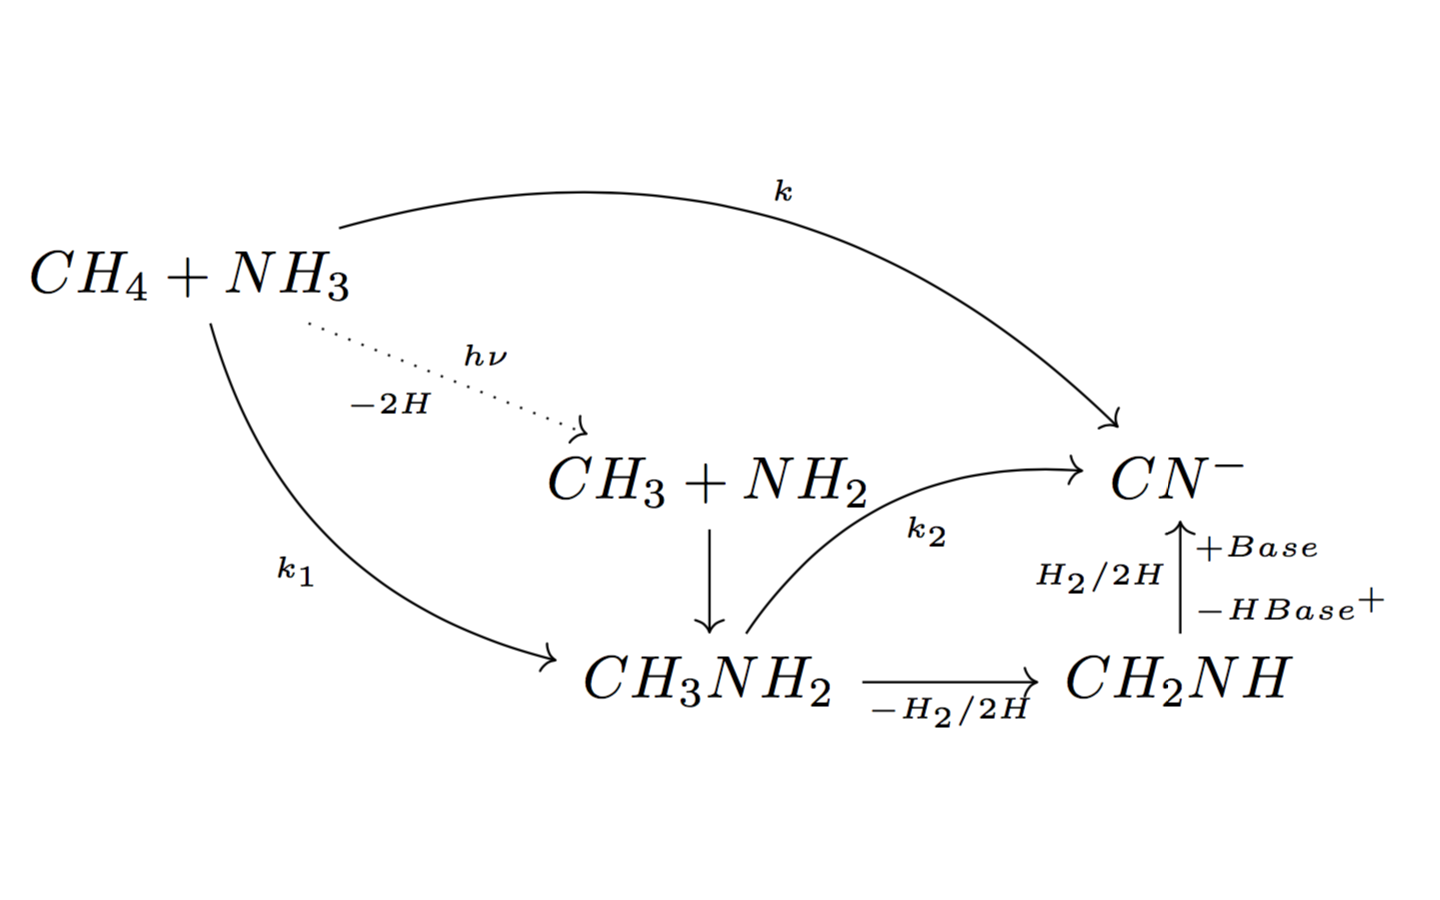
\includegraphics[width=\textwidth]{figures/chapter3/CNmechanism}
\caption{The formation mechanism of CN$^-$ proposed by Kim and Kaiser(2011). }
\label{fig:CNmechanism}
\end{figure}

The formation mechanism of CN$^-$ is proposed by Kim and Kaiser(2011). CH$_4$ and NH$_3$ irradiated by photon to become CH$_3$ and NH$_2$ radical (figure \ref{CNmechanism}, followed by propagation and recombination of radicals becoming CH$_3$NH$_2$ and dehydrogenation and acid-base reaction to form CN$^-$.
This formation mechanism also applies in our photon irradiation experiments because we can also detect the methylamine during our warm-up phase. The ion fragment with m/z=31 is assigned as CH$_3$NH$_2$$^+$ and detectable in all ratios of our CH$_4$+NH$_3$ experiments (figure \ref{Mass31}).

\begin{figure}
\centering
\includegraphics[width=\textwidth]{figures/chapter3/Mass31.eps}
\caption{The m/z=31 detected by QMS during warm-up with heating rate 1 K/min in different configurations of ice mixtures.
 }
\label{fig:CNmechanism}
\end{figure}

By the deviation performed in section \ref{sec:Reaction_Rate_Laws}, we have a rate equation for consecutive reactions \ref{eq:rate7}. With one of the reactant larger than another, we applied the pseudo first order assumption. With equation \ref{eq:rate7}, we fitted the formation of CN$^-$ (figure \ref{fig:CNrate})and found that one of the rate constant is always larger than the other in all of the ratios. The fitting results are averaged by more than two experiments and are shown in table \ref{tab:CNrate}./Users/Lily/thesis


\begin{figure}
\centering
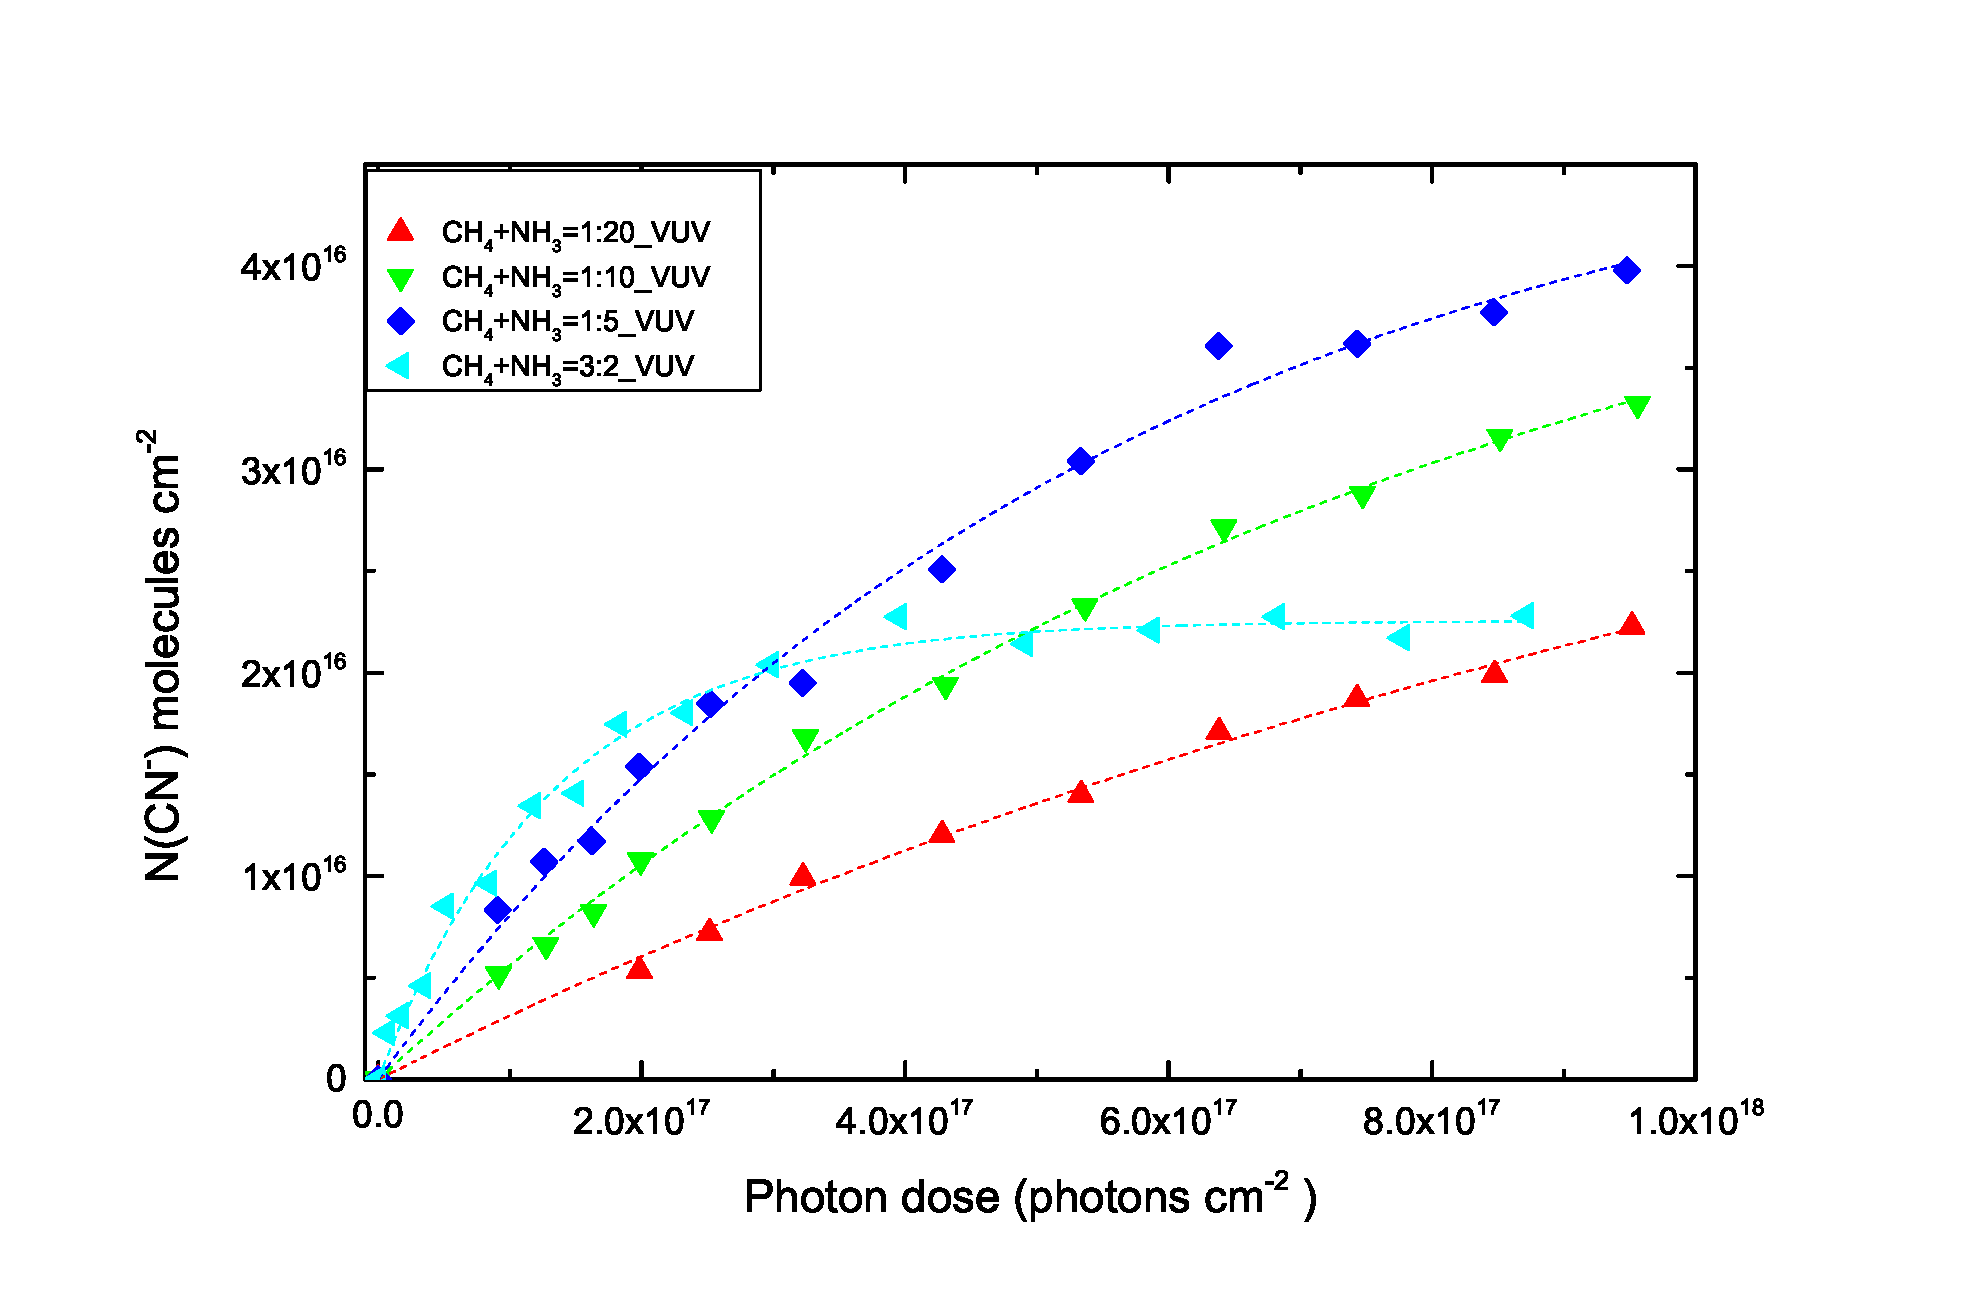
\includegraphics[width=\textwidth]{figures/chapter3/Overall_CN_rate.eps}
\caption{The column density of CN$^-$ accumulated when different configurations of CH$_4$ + NH$_3$ ice mixtures are irradiated by VUV photons provided by MDHL. The dotted lines are fits of column densities by equation \ref{eq:rate7}.}
\label{fig:CNrate}
\end{figure}

\begin{table}[htbp]
\caption{The fitting results of CN$^-$ by equation \ref{eq:rate7}}
\label{tab:CNrate}
\begin{tabular}{cccc}
\hline
\hline
Ratio of CH$_4$+NH$_3$ & A (x10$^{16}$ molecules cm$^{-2}$) & k$_1$ (x10$^{-18}$ photon$^{-1}$) & k$_2$ (photon$^{-1}$)\\
\hline
1:20 & 4.75 $\pm$ 0.40 & 0.70 $\pm$ 0.09 & >1 \\
1:10 & 4.51 $\pm$ 0.18 & 1.33 $\pm$ 0.13 & >1 \\
1:5 & 4.61 $\pm$ 0.18 & 1.93 $\pm$ 0.19 & >1 \\
3:2 & 2.24 $\pm$ 0.03 & 8.21 $\pm$ 0.70 & >1 \\
\hline
\end{tabular}
\end{table}

